%%=====================================================================
%%  RT-IIPF -- 6-page IEEE conference cut
%%  Extended journal version: main.tex (unmodified)
%%  Build:  pdflatex conference && bibtex conference && pdflatex conference x2
%%=====================================================================
\documentclass[conference]{IEEEtran}
\IEEEoverridecommandlockouts

\usepackage{cite}
\usepackage{amsmath,amssymb,amsfonts}
\usepackage{graphicx}
\usepackage{booktabs}
\usepackage{array}
\usepackage{tikz}
\usetikzlibrary{positioning,arrows.meta,fit,backgrounds}
\usepackage{url}

\newcommand{\INR}[1]{\mbox{INR~#1}}

\begin{document}

\title{RT-IIPF: A Real-Time Inline Payment Fraud Mitigation
Framework Using Fused Isolation Forests and Local Outlier Factors}

\author{
\IEEEauthorblockN{[Author One]}
\IEEEauthorblockA{\textit{School of Computing} \\
\textit{Sathyabama Institute of Science and Technology}\\
Chennai, India \\
[email@domain]}
\and
\IEEEauthorblockN{[Author Two]}
\IEEEauthorblockA{\textit{School of Computing} \\
\textit{Sathyabama Institute of Science and Technology}\\
Chennai, India \\
[email@domain]}
}

\maketitle

\begin{abstract}
Instant payment networks settle irrevocably, so a control that scores a
transaction after commit acts on funds that have already moved. This
paper presents RT-IIPF, which evaluates a payment inside the database
transaction while both ledger rows are held under
\texttt{PESSIMISTIC\_WRITE} locks and the debit remains uncommitted; a
fraudulent transfer is rolled back atomically and never persists in the
ledger. Scoring fuses three tiers: rules whose thresholds are derived
from training-distribution quantiles, an Isolation Forest ($M=200$,
$\psi=256$), and a Local Outlier Factor estimator ($k=20$) over a fixed
$40{,}000$-point reference set in $67$ dimensions. The fused score is
$\max(0.2\,S_{\mathrm{IF}} + 0.8\,S_{\mathrm{LOF}},\,R)$, thresholded at
$\tau = 0.802$ fixed by a matched false-positive-rate sweep at
$\mathrm{FPR}=0.0086$. On $50{,}000$ clean and $400$ injected
transactions the deployed configuration attains recall $0.745$,
precision $0.380$, and F1 $0.503$. Account lockout commits through an
independent \texttt{REQUIRES\_NEW} transaction and survives the ledger
rollback. Inference costs $17.3$\,ms and end-to-end switch latency is
$22.4$\,ms at unit concurrency, with single-worker p95 within a
$500$\,ms budget up to $25$ concurrent clients. Contended and
uncontended throughput are statistically indistinguishable, so the
system is not lock-bound.
\end{abstract}

\begin{IEEEkeywords}
Payment systems, anomaly detection, isolation forest, local outlier
factor, real-time switches, transactional rollback.
\end{IEEEkeywords}

%%=====================================================================
%%---------------------------------------------------------------------
%%  PAGE BUDGET NOTE
%%  Estimated 6.0-6.4 pages. The estimate is a heuristic (words/page),
%%  NOT a compile -- no TeX engine was available when this was written.
%%  Check the real page count on the first build. If it runs over, apply
%%  these cuts in order; each is self-contained and loses no result:
%%
%%   1. Delete Fig.~\ref{fig:lifecycle} (the tikzpicture block) and the
%%      sentence referring to it in Sec.~V-D.          saves ~0.45 pg
%%   2. In Sec.~II, delete the final paragraph (prior-work confusion
%%      matrix); keep the \cite{kumar2026} in Sec. I.  saves ~0.10 pg
%%   3. In Sec.~VI, delete the "Limitations:" paragraph and fold the
%%      two key ones into the preceding paragraph.     saves ~0.10 pg
%%   4. In Sec.~V-D, delete the final sentence on the 512 MB container.
%%                                                     saves ~0.05 pg
%%  Do NOT cut: Tables I-II, Eqs. (6)-(8), or the C1-C3 list.
%%---------------------------------------------------------------------
%%=====================================================================
\section{Introduction}
\label{sec:introduction}

Instant retail payment networks settle irrevocably. Once a Unified
Payments Interface (UPI) transfer commits, funds reach the beneficiary
within seconds and recovery depends on intermediary cooperation rather
than reversal. The interval in which a payment can be stopped at zero
cost is the interval before the database transaction commits, measured
in milliseconds. Most deployed controls do not operate inside it: they
score after settlement, converting a detection problem into a recovery
problem.

An inline control consumes part of the switch's processing window and,
because it executes while ledger rows are held under write locks, also
extends the period those accounts are unavailable. Its cost is
therefore twofold: response latency and lock occupancy. We adopt a
$500$\,ms round-trip budget as the design target and report measured
latency against it.\footnote{This is the present work's engineering
budget; a citation to the governing network specification should
replace this note before submission.}

Batch pipelines impose no latency on the authorisation path but act on
funds already moved. Deep sequential~\cite{jurgovsky2018} and
graph~\cite{dou2020} models capture behavioural context, but their
inference cost and their need to assemble a history or neighbourhood
at scoring time place them outside a millisecond window held under a
lock; both are supervised, requiring labels scarce precisely when a
pattern is novel. The gap is a detector cheap enough to run inside the
lock window, needing no labels, producing a decision the transaction
manager can act on before commit. This paper contributes:

\textbf{C1.} An inline hybrid pipeline combining a deterministic rule
tier with an Isolation Forest and a Local Outlier Factor estimator
($k=20$, $|\mathcal{R}|=40{,}000$, $d=67$), fused by a weighted blend
floored by rule risk and thresholded at $\tau=0.802$. The pipeline is
stateless and deterministic, so verdicts are reproducible during audit.

\textbf{C2.} A decoupled switch preserving a security invariant under
rollback: on a fraud verdict the account lock and audit record commit
through an independent \texttt{REQUIRES\_NEW} transaction completing
\emph{before} the financial transaction rolls back, so security state
persists while the ledger is left arithmetically unchanged.

\textbf{C3.} Measurement of the inline cost, including negative
results. Single-worker p95 stays within budget to $25$ concurrent
clients and exceeds it at $50$. We report that the Isolation Forest
tier changes no verdict on our evaluation set, and that rule escalation
reduces precision without increasing recall.

%%=====================================================================
\section{Related Work}
\label{sec:relatedwork}

\textbf{Rule engines} remain the default inline control for
architectural rather than statistical reasons: threshold conjunctions
evaluate in constant time, hold no model state, emit a reason code, and
fail reconstructibly. Surveys record them as the component that
executes on the authorisation path, with learned models
downstream~\cite{abdallah2016}. Their limits are equally established---a
fixed predicate set encodes only attacks known at authoring time,
absolute thresholds drift as the amount distribution shifts, and a
conjunction over individual attributes cannot express an anomaly
distributed \emph{across} attributes. We retain a rule tier but narrow
its role: thresholds are training quantiles, and the tier acts as a
lower bound on risk rather than as the primary classifier.

\textbf{Supervised and deep models.} Gradient-boosted trees are the
standard tabular baseline~\cite{chen2016}; sequential~\cite{jurgovsky2018}
and graph~\cite{dou2020} architectures add behavioural and relational
context~\cite{adewumi2017}. Three properties bear jointly on inline
use. All need confirmed labels, produced over days to weeks, so the
label set is empty exactly when a novel pattern must be caught. All
need a retraining loop whose integrity depends on annotation
quality---a fragility our corpus exhibits, its \texttt{fraud\_flag}
column yielding ROC-AUC~$\approx 0.48$ against every detector we
evaluated. And sequential and graph variants must assemble a history or
neighbourhood at scoring time, adding database work to a window the
detector already extends. The unsupervised per-transaction formulation
here avoids all three, at the cost of detecting \emph{atypicality}
rather than \emph{fraud} and of blindness to velocity attacks, which we
quantify with a negative control.

\textbf{Unsupervised ensembles.} Isolation Forest~\cite{liu2008} scores
by expected path length under random axis-parallel partitioning,
costing $\mathcal{O}(M\log\psi)$ independent of training-set size. Its
power degrades where anomalies are local rather than globally extreme
and, as Section~\ref{sec:evaluation} measures, where the representation
is dominated by sparse one-hot indicators. Local Outlier
Factor~\cite{breunig2000} covers that case via local density contrast
with the inverse cost structure: under brute-force search construction
is $\mathcal{O}(N^{2}d)$ and each query $\mathcal{O}(Nd)$, so over our
$200{,}000$-row partition the query term alone would dominate the lock
window. One-class SVMs~\cite{scholkopf2001} pose a comparable obstacle.
With no uniformly dominant method~\cite{campos2016}, combination is
preferable to selection. We bound the LOF term by fixing
$|\mathcal{R}|=40{,}000$ points sampled once and held resident.

The closest prior work scores UPI records from the same public
source~\cite{kumar2026}, but issues a step-up challenge \emph{after}
the model clears a transaction, in application flow, and reports no
latency. Its published confusion matrix ($\mathrm{TN}{=}75$,
$\mathrm{FP}{=}6$, $\mathrm{FN}{=}85$, $\mathrm{TP}{=}14$) implies
accuracy $49.4\%$ and recall $14.1\%$, disagreeing with the accuracy
stated in the same paper. We therefore avoid accuracy entirely: at our
$0.79\%$ prevalence a detector flagging nothing scores $99.21\%$.

%%=====================================================================
\section{Hybrid Inference Pipeline}
\label{sec:methodology}

\subsection{Features and Embedding}
A payment is represented by $13$ components: three numeric (amount,
hour, weekend flag) and ten categorical (transaction type, merchant
category, sender and receiver age group, sender state, sender and
receiver bank, device type, network type, day of week). The payer
supplies three via the form, the client runtime two as background
telemetry, and the switch resolves eight from its own records and
clock when the rows are locked. Nothing comes from the payee or
depends on the outcome being scored.

Both learned tiers share an embedding $\Phi$ fitted once on the
training partition: numeric standardised, categorical one-hot
expanded, unseen levels encoding to zero so the service stays total
over arbitrary input. The one-hot blocks add $64$ coordinates, so
\begin{equation}
d = 3 + 64 = 67 ,
\label{eq:dim}
\end{equation}
of which $64$ are binary and exactly $10$ non-zero per record---a
geometry that governs both tiers. Training uses $200{,}000$ rows, an
$80\%$ split of a $250{,}000$-row corpus under seed~$42$.

\subsection{Learned Tiers}
We fit $M=200$ isolation trees with subsample size $\psi=256$ and
contamination $0.002$. The canonical isolation score and its
path-length normalisation follow Liu~et~al.~\cite{liu2008} and are not
restated. Writing $a_{\mathrm{IF}}$ for the implementation's
offset-shifted score---an affine, order-preserving transform---we
calibrate onto $[0,1]$ by
\begin{equation}
S_{\mathrm{IF}} = \operatorname{clip}_{[0,1]}\!\left(
\frac{a_{\mathrm{IF}} - \alpha^{-}_{\mathrm{IF}}}
     {\alpha^{+}_{\mathrm{IF}} - \alpha^{-}_{\mathrm{IF}}}\right),
\label{eq:S_IF}
\end{equation}
with $\alpha^{-}_{\mathrm{IF}}=-0.108678$ the training minimum and
$\alpha^{+}_{\mathrm{IF}}=0.008023$ the $99.95$th percentile; anchoring
above the maximum prevents one outlier compressing the range.

For Tier~3 we draw $|\mathcal{R}|=40{,}000$ points uniformly without
replacement under seed~$42$ and fit a novelty-mode estimator with
$k=20$ under the Euclidean metric. With $\mathrm{lrd}_{k}$ the local
reachability density~\cite{breunig2000},
\begin{equation}
\mathrm{LOF}_{k}(\mathbf{z}) = \frac{1}{k}
\sum_{\mathbf{o}\in N_{k}(\mathbf{z})}
\frac{\mathrm{lrd}_{k}(\mathbf{o})}{\mathrm{lrd}_{k}(\mathbf{z})} ,
\label{eq:lof}
\end{equation}
values above unity indicating a locally sparse neighbourhood. With
$a_{\mathrm{LOF}} = \mathrm{LOF}_{k} - 1.5$,
\begin{equation}
S_{\mathrm{LOF}} = \operatorname{clip}_{[0,1]}\!\left(
\frac{a_{\mathrm{LOF}} - \alpha^{-}_{\mathrm{LOF}}}
     {\alpha^{+}_{\mathrm{LOF}} - \alpha^{-}_{\mathrm{LOF}}}\right),
\label{eq:S_LOF}
\end{equation}
$\alpha^{-}_{\mathrm{LOF}}=-0.550359$,
$\alpha^{+}_{\mathrm{LOF}}=-0.351704$, computed over $\mathcal{R}$.

\subsection{Rule Tier, Fusion and Decision}
Beyond the training support \eqref{eq:S_IF} and \eqref{eq:S_LOF} clip
at unity and stop discriminating; Tier~1 supplies a path independent of
that support and emits a reason code. Its thresholds are training
quantiles, not authored constants:
$\theta_{\mathrm{ext}}=Q_{99.9}=\INR{16{,}450}$,
$\theta_{\mathrm{high}}=Q_{99.0}=\INR{8{,}998}$,
$\theta_{\mathrm{tick}}=Q_{99.5}=\INR{11{,}136}$. With $a,\eta,
\tau_{\mathrm{t}},m,v$ the amount, hour, type, category and device, and
$\Sigma = [\tau_{\mathrm{t}}{=}\texttt{Recharge}] \vee
[m\in\{\texttt{Grocery},\texttt{Food},\texttt{Transport}\}]$, the
predicates and weights are
$r_{1}\!:a \geq \theta_{\mathrm{ext}}$ $(0.55)$;
$r_{2}\!:a \geq \theta_{\mathrm{high}} \wedge \eta \leq 5$ $(0.30)$;
$r_{3}\!:\Sigma \wedge a \geq \theta_{\mathrm{tick}}$ $(0.35)$;
$r_{4}\!:a \geq \theta_{\mathrm{high}} \wedge v{=}\texttt{Web}$
$(0.20)$, giving
\begin{equation}
R = \operatorname{clip}_{[0,1]}\!\Big(\textstyle\sum_{i} w_{i}
\mathbb{1}[r_{i}]\Big),
\quad
H = r_{1} \vee \Big(\textstyle\sum_{i}\mathbb{1}[r_{i}] \geq 2\Big).
\label{eq:rules}
\end{equation}
The flag $H$ encodes two arguments for blocking: one predicate strong
enough alone, or corroboration across independent predicates.

The learned tiers blend convexly with weights $0.20$ and $0.80$ fixed
by a sweep on the injected set, and the rule tier enters as a
\emph{floor} rather than a third addend:
\begin{equation}
S = \operatorname{clip}_{[0,1]}\!\Big(\max\big\{
0.2\,S_{\mathrm{IF}} + 0.8\,S_{\mathrm{LOF}},\; R \big\}\Big),
\label{eq:fused}
\end{equation}
guaranteeing $S \geq R$ pointwise, so no combination of learned scores
can place a transaction below the risk the rules assign it---the
cancellation a weighted sum would permit. The verdict is
\begin{equation}
\hat{y} = \mathbb{1}\!\left[\, S \geq \tau \;\vee\; H \,\right],
\qquad \tau = 0.802 ,
\label{eq:decide}
\end{equation}
$\tau$ fixed by a matched-FPR sweep and serialised in the bundle, so
the deployed boundary equals the evaluated one. The disjunction is not
redundant: $\{r_{2},r_{4}\}$ gives $R = 0.50 < \tau$ while satisfying
$H$. Equation~\eqref{eq:decide} involves no randomness, request-order
dependence or mutable state---detectors are loaded once and
read-only---so identical inputs yield identical verdicts across
processes and restarts, which audit requires.

%%=====================================================================
\section{Inline Transaction Switch}
\label{sec:architecture}

A Java~21 / Spring~Boot switch owns authentication, ledger state, locks
and the commit decision, embedding an H2 engine in-process so no
network hop separates the application from its locks. A containerised
Python / FastAPI node owns inference, holding the preprocessor, both
detectors and the $40{,}000\times 67$ reference matrix resident. It is
stateless---no writes, no distributed transaction---so it cannot
corrupt ledger state under any failure mode; its worst contribution is
unavailability.

The scoring hop is \emph{synchronous and blocking}: a requirement, not
a shortcut. The switch issues a blocking call from inside an open
\texttt{@Transactional} method while holding write locks on both
balance rows, suspending the thread for the round trip. An asynchronous
hop would place the verdict after the commit boundary, reducing the
design to post-settlement detection with extra latency. The switch
guarantees $t_{\mathrm{lock}} < t_{\mathrm{score}} <
t_{\mathrm{commit}}$ for every committing transaction.

Both rows are acquired under \texttt{PESSIMISTIC\_WRITE}; optimistic
versioning is unsuitable because retry-on-conflict would re-invoke the
scorer, multiplying the dominant cost term. Locks are taken in
ascending user-identifier order, a total order eliminating the cyclic
wait-for condition, so opposing concurrent payments serialise rather
than deadlock---necessary because each transaction holds its first lock
across a network round trip. Three terminal states persist:
\texttt{SUCCESS} ($\hat{y}{=}0$, HTTP~200) commits both legs;
\texttt{BLOCKED\_FRAUD} ($\hat{y}{=}1$, HTTP~403) rolls back and locks
the payer; \texttt{FAILED} covers pre-verdict rejections (4xx) and
scorer unavailability (503).

\textbf{Security boundary.} A rollback discarding the fraudulent debit
would, under one transaction, also discard the evidence and the lock
raised in response. Let $T_{f}$ be the financial transaction and
$T_{s}$ a second declared \texttt{Propagation.REQUIRES\_NEW}. On
$\hat{y}{=}1$ the switch suspends $T_{f}$, opens $T_{s}$ on a separate
connection, sets the payer's lock flag and inserts the
\texttt{BLOCKED\_FRAUD} audit row, commits $T_{s}$ at $t_{1}$, then
resumes $T_{f}$ and raises the fraud exception, rolling back at
$t_{2}>t_{1}$. Because $T_{s}$ commits strictly first on an independent
connection,
\begin{equation}
\mathrm{eff}(T_{s}) \neq \emptyset
\;\wedge\;
\mathrm{eff}(T_{f}) = \emptyset ,
\label{eq:invariant}
\end{equation}
so lock and audit persist while balances are untouched. The ordering is
not interchangeable: committing $T_{s}$ after the exception would place
the write on an unwinding stack, and nesting it inside $T_{f}$ would
discard it with the debit. We verified \eqref{eq:invariant} by
observing the audit row count increment across a rollback while both
balances retained pre-transaction values.

\textbf{Fail-closed and resources.} Every non-success outcome raises
one scoring-unavailable fault yielding HTTP~503 and rollback; no path
commits an unscored payment. The alternative is exploitable: a system
admitting payments when its scorer is unreachable can be opened by
denying service to the scorer, which is cheaper than defeating the
detector. The read timeout ($1500$\,ms) bounds lock-hold time, not
merely request duration. Each scorer worker is a separate process
holding its own bundle copy at $184$\,MB resident, $220$--$250$\,MB
with the server; against a $512$\,MB container limit this admits
$W_{\max}=2$, and we set $W=1$ for headroom during the neighbour query.
The reference matrix is read-only after startup, so handlers are
race-free and scoring stays deterministic.
\begin{figure}[t]
\centering
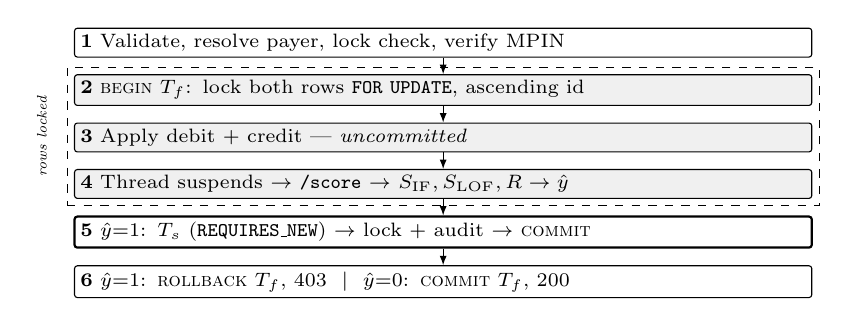
\begin{tikzpicture}[
  node distance=2.1mm, font=\scriptsize,
  box/.style={draw, rounded corners=1pt, align=left,
              text width=0.76\columnwidth, inner sep=2.1pt},
  crit/.style={box, fill=black!6},
  blk/.style={box, draw=black, thick},
  arrow/.style={-{Latex[length=1.2mm]}}
]
\node[box]  (n1) {\textbf{1}~Validate, resolve payer, lock check, verify MPIN};
\node[crit, below=of n1] (n2) {\textbf{2}~\textsc{begin} $T_{f}$: lock both rows \texttt{FOR UPDATE}, ascending id};
\node[crit, below=of n2] (n3) {\textbf{3}~Apply debit $+$ credit --- \emph{uncommitted}};
\node[crit, below=of n3] (n4) {\textbf{4}~Thread suspends $\rightarrow$ \texttt{/score} $\rightarrow$ $S_{\mathrm{IF}}, S_{\mathrm{LOF}}, R \rightarrow \hat{y}$};
\node[blk,  below=of n4] (n5) {\textbf{5}~$\hat{y}{=}1$: $T_{s}$ (\texttt{REQUIRES\_NEW}) $\rightarrow$ lock $+$ audit $\rightarrow$ \textsc{commit}};
\node[box,  below=of n5] (n6) {\textbf{6}~$\hat{y}{=}1$: \textsc{rollback} $T_{f}$, 403 ~\textbar~ $\hat{y}{=}0$: \textsc{commit} $T_{f}$, 200};
\foreach \a/\b in {n1/n2, n2/n3, n3/n4, n4/n5, n5/n6}
  \draw[arrow] (\a) -- (\b);
\begin{scope}[on background layer]
  \node[draw, dashed, fit=(n2)(n3)(n4), inner sep=2.5pt] (win) {};
\end{scope}
\node[rotate=90, anchor=south, font=\tiny\itshape]
  at ([xshift=-1.3mm]win.west) {rows locked};
\end{tikzpicture}
\caption{Execution lifecycle. Steps 2--4 hold both balance rows under
\texttt{PESSIMISTIC\_WRITE}. Step~5 commits on an independent
connection and survives the rollback in step~6, establishing
\eqref{eq:invariant}.}
\label{fig:lifecycle}
\end{figure}
%%=====================================================================
\section{Empirical Evaluation}
\label{sec:evaluation}

\subsection{Setup}
An $80/20$ split of the $250{,}000$-record corpus under seed~$42$
yields $200{,}000$ training and $50{,}000$ held-out clean rows. We do
not use the shipped \texttt{fraud\_flag} as ground truth: it yields
ROC-AUC~$\approx 0.48$, indistinguishable from random, so supervised
metrics against it would measure the label rather than the detector.
Instead we sample real clean rows and overwrite only the fields
defining each archetype, leaving the rest at sampled values so
synthetics are not separable by a generation artefact. Four archetypes
of $100$ instances give $400$ injected transactions at $0.79\%$
prevalence: (A) off-hour drain, $\mathcal{U}(25\mathrm{k},60\mathrm{k})$,
hour $\in\{1..4\}$, Web; (B) velocity spike \emph{(negative control)},
$\mathcal{U}(2\mathrm{k},6\mathrm{k})$, business hours, Android;
(C) category anomaly, $\mathcal{U}(50\mathrm{k},100\mathrm{k})$,
Grocery, daytime; (D) context anomaly,
$\mathcal{U}(2\mathrm{k},9\mathrm{k})$, hour $\in\{0..4\}$, Web, WiFi.
Archetype~B detects methodological error: velocity is an arrival-rate
property no per-transaction vector carries, so appreciable recall
on~B would indicate leakage. Sweeping $S$ to $\mathrm{FPR}=0.0086$
returns $\tau=0.802$; all comparisons use this matched FPR.

\begin{table}[t]
\centering
\caption{Tier ablation at matched $\mathrm{FPR}=0.0086$.
$\mathrm{FDR}=1-\mathrm{P}$.}
\label{tab:ablation}
\renewcommand{\arraystretch}{1.2}
\footnotesize
\setlength{\tabcolsep}{4pt}
\begin{tabular}{@{}lccccc@{}}
\toprule
\textbf{Configuration} & \textbf{P} & \textbf{R} & \textbf{F1} & \textbf{FDR} & \textbf{AUC} \\
\midrule
(a) Tier-1 rules only$^{\dagger}$          & $0.738$ & $0.500$ & $0.596$ & $0.262$ & --- \\
(b) Isolation Forest only                  & $0.121$ & $0.147$ & $0.133$ & $0.879$ & $0.7231$ \\
(c) LOF only ($k=20$)                      & $0.409$ & $0.745$ & $0.528$ & $0.591$ & $0.8959$ \\
(d) Fusion, no escalation                  & $0.409$ & $0.745$ & $0.528$ & $0.591$ & $0.8812$ \\
\midrule
(e) \textbf{RT-IIPF deployed}$^{\ddagger}$ & $0.380$ & $0.745$ & $0.503$ & $0.620$ & --- \\
\bottomrule
\end{tabular}

\vspace{2pt}
{\footnotesize\raggedright
$^{\dagger}$Deterministic binary decision; FPR $0.0014$, not tunable.
$^{\ddagger}$Fusion \eqref{eq:fused} with escalation \eqref{eq:rules};
FPR $0.0097$.\par}
\end{table}

\subsection{Tier Ablation}
Table~\ref{tab:ablation} yields three findings, two negative.

\emph{The density tier carries detection.} Configuration~(c) raises
recall from $0.147$ to $0.745$ over~(b) at identical FPR, a factor of
$5.07$. The cause is the geometry of \eqref{eq:dim}: with $64$ of $67$
coordinates binary and $10$ non-zero per record, axis-parallel random
splits fall predominantly on all-zero coordinates and isolate little,
whereas \eqref{eq:lof} operates on the full vector at once.

\emph{The forest contributes no detection.} Configurations~(c) and~(d)
agree to three decimals on precision, recall and F1, and their
per-archetype recalls coincide exactly---A~$1.00$, B~$0.01$, C~$1.00$,
D~$0.97$---against the forest's $0.26$, $0.00$, $0.07$, $0.26$. Adding
the forest at weight $0.20$ changes no verdict while reducing AUC from
$0.8959$ to $0.8812$. On one-hot-dominated payment features a
partition-based detector fused with a density-based one supplies no
incremental detection, at the largest single share of inference cost.

\emph{Escalation costs precision without adding recall.}
Configuration~(e) holds recall at $0.745$ while precision falls to
$0.380$ and FDR rises to $0.620$. We retain the rules on grounds this
set cannot measure---validity beyond the training support, reason-code
emission, degraded-mode operation---quantified below. Archetype~B
returns $0.01$, within noise of the expected zero, supporting the
injection procedure. Excluding~B the detectable population is $300$, of
which the deployed system identifies $297$ ($99.0\%$ of the ceiling);
aggregate recall is bounded above by $0.75$ by construction. We report
the unadjusted figure and state the bound.

\begin{table}[t]
\centering
\caption{Amount sweep, all other features held constant (P2M, Grocery,
Web, 4G, hour~18, weekday). Amounts in INR.}
\label{tab:sweep}
\renewcommand{\arraystretch}{1.15}
\footnotesize
\setlength{\tabcolsep}{4pt}
\begin{tabular}{@{}rccccl@{}}
\toprule
\textbf{Amount} & $S_{\mathrm{IF}}$ & $S_{\mathrm{LOF}}$ & $R$ & $S$ & \textbf{Verdict} \\
\midrule
$50$            & $0.467$ & $0.340$ & $0.00$ & $0.365$ & ALLOW \\
$1{,}000$       & $0.461$ & $0.357$ & $0.00$ & $0.377$ & ALLOW \\
$5{,}000$       & $0.531$ & $0.814$ & $0.00$ & $0.757$ & ALLOW \\
$8{,}998^{a}$   & $0.593$ & $0.568$ & $0.00$ & $0.573$ & ALLOW \\
$11{,}136^{b}$  & $0.617$ & $0.519$ & $0.20$ & $0.538$ & ALLOW \\
$16{,}450^{c}$  & $0.617$ & $0.474$ & $0.55$ & $0.550$ & \textbf{BLOCK} \\
$20{,}000$      & $0.617$ & $0.537$ & $1.00$ & $1.000$ & \textbf{BLOCK} \\
$50{,}000$      & $0.617$ & $1.000$ & $1.00$ & $1.000$ & \textbf{BLOCK} \\
\bottomrule
\end{tabular}

\vspace{2pt}
{\footnotesize\raggedright
$^{a}\theta_{\mathrm{high}}$, $^{b}\theta_{\mathrm{tick}}$,
$^{c}\theta_{\mathrm{ext}}$.\par}
\end{table}

\subsection{Decision Boundary Across the Amount Domain}
Table~\ref{tab:sweep} varies only the amount. First, \emph{the learned
score is not monotone in amount}: $S_{\mathrm{LOF}}$ reaches $0.814$ at
\INR{5{,}000} and falls to $0.519$ at \INR{11{,}136}, a larger transfer
in the same context. This is correct for a density statistic---%
\INR{5{,}000} occupies a thinner region of the Grocery/P2M
population---but it means a policy requiring risk not to decrease with
amount cannot be expressed by the learned tiers. Column~$R$ is monotone
by construction and supplies that guarantee. Second, \emph{the decision
disjunction is not redundant}: at \INR{16{,}450} the system blocks with
$S=0.550<\tau$, the verdict produced entirely by the hard-rule branch
of \eqref{eq:decide}; thresholding on $S$ alone would admit it. The
\INR{50} and \INR{50{,}000} endpoints share an identical channel
context and differ only in amount yet receive opposite verdicts, so the
boundary is driven by the transaction rather than the channel.

\subsection{Latency and Lock Contention}
On the laboratory host over $n=300$ warm iterations, inference totals
$17.33$\,ms: Isolation Forest $9.55$\,ms ($55.1\%$), preprocessor
$3.80$, LOF $3.18$, frame construction $0.61$, rules $0.19$. The forest
takes the largest share while contributing no detection; removing it
would reduce inference to roughly $7.8$\,ms at unchanged recall. At
concurrency~$1$ the switch completes a payment in mean $22.4$\,ms
(p95~$23.8$, p99~$25.3$), attributing $\approx 5.1$\,ms to switch-side
work. The lock-hold window spans steps 2--4 of
Fig.~\ref{fig:lifecycle}, bounded by
\begin{equation}
17.3~\mathrm{ms} \;\lesssim\; W_{\mathrm{lock}} \;\lesssim\; 22.4~\mathrm{ms},
\label{eq:lockwindow}
\end{equation}
with a hard ceiling of $1500$\,ms from the read timeout. This is what
the architecture trades for pre-commit interception.

Comparing an uncontended workload, each client holding a distinct
account pair, against a contended one where all compete for an
overlapping set, throughput was $44.5$ vs $47.2$~TPS at one client,
$49.2$ vs $50.4$ at ten, $49.5$ vs $50.6$ at $25$ and $50.0$ vs $50.8$
at $50$---ratios of $1.016$--$1.061$. Every ratio equals or exceeds
unity, so forcing all clients onto the same rows produced no measurable
penalty: the system is not lock-bound. The binding constraint is the
single-worker scorer, which plateaus near $50$\,TPS and saturates
before lock queuing becomes observable; no deadlock occurred. Measured
p95 stays within budget to $25$ clients ($374.5$\,ms) and exceeds it at
$50$ ($864.2$\,ms). A p99 of $3.9$--$4.0$\,s appears at
concurrency~$\geq 10$ in \emph{both} workloads while p95 stays below
$65$\,ms at ten; its equal magnitude under both conditions indicates
connection queuing against the saturated scorer, not lock waiting. On a
$512$\,MB shared-CPU container warm inference measures $178.1$\,ms
($n=9$), roughly $10\times$ the laboratory figure---CPU provisioning,
not algorithm or transport.

%%=====================================================================
\section{Conclusion and Future Work}
\label{sec:conclusion}

We implemented and measured a fraud control executing inside the
database transaction, while ledger rows are locked and the debit
uncommitted. A fraudulent transfer is rolled back atomically and never
persists, while the lock and audit record commit independently and
survive that rollback---\eqref{eq:invariant}, verified experimentally.
The inline cost is $17.3$\,ms of inference within a $22.4$\,ms path at
unit concurrency and the lock window of \eqref{eq:lockwindow}.

The division of labour is not the one the design anticipated.
Detection is carried entirely by the density estimator: LOF alone
matches the fused configuration to three decimals, while the forest
changes no verdict at $55.1\%$ of inference cost. The rule tier buys
bounds rather than recall---it costs precision ($0.409 \rightarrow
0.380$) but remains valid beyond the training support, emits reason
codes, and enforces the amount-monotonicity the learned tiers
demonstrably lack, binding at the \INR{16{,}450} point where
$S=0.550<\tau$. The system is not lock-bound; the scorer is the
constraint.

Limitations: the feature vector is per-transaction, so velocity attacks
are undetectable by construction (archetype~B, recall $0.01$); ground
truth is synthetic, the corpus labels being uninformative; LOF
calibration anchors are computed in-sample on $\mathcal{R}$; the
embedded database preserves the audit trail for the process lifetime
only; and results derive from one corpus and one geography.

Four directions follow. Multiplexed gRPC over Protocol Buffers targets
the $3.9$--$4.0$\,s p99---connection queuing, not lock waiting---by
removing connection establishment, head-of-line blocking and JSON
serialisation from a path holding locks throughout. The reference set
is frozen at training time, so the density estimate ages under drift
while $\mathcal{O}(|\mathcal{R}|d)$ bounds its growth; approximate
nearest-neighbour indexing and a rolling-window sharded set both apply,
raising consistency questions between replicas holding different
reference states while \eqref{eq:decide} requires reproducible
verdicts. Persisting the device signature the client already captures
but the model never receives would admit an \texttt{is\_new\_device}
feature addressing the social-engineering case. Finally, routing scores
just below $\tau$ to out-of-band re-authentication would convert part
of the $0.620$ false discovery rate into a challenge rather than a
block.

%%=====================================================================
\bibliographystyle{IEEEtran}
\bibliography{references}

\end{document}
